\graphicspath{{chapters/munthe/graphics/}}


\title{Growth and Remodelling Package in FEniCSx}

\author{Karl Munthe, Henrik Finsberg, Samuel Wall, Joakim Sundnes}

\institute{K. Munthe \at Simula Research Laboratory, Oslo, Norway and \\ Department of Informatics, University of Oslo, Norway, \email{karlfredrik@simula.no}
\and
H. Finsberg \at Simula Research Laboratory, Oslo, Norway
\and
S. Wall \at Simula Research Laboratory, Oslo, Norway
\and
J. Sundnes \at Simula Research Laboratory, Oslo, Norway and \\ Department of Informatics, University of Oslo, Norway}

\maketitle
\abstract{The heart is a dynamic organ that changes its size and shape to regulate its behaviour to the demands of the body, which can change for example through body growth, exercise, or the onset of a disease. Different models have been proposed to try to capture various types of cardiac growth resulting from mechanical stimuli, but the models have rarely been compared systematically. In this manuscript we present a framework implemented in FEniCSx that allows one to quickly run simulations of growth and remodelling with different material models and different growth laws. We present and compare the growth predicted by each model for a set of simple experiments, and compare the results to the relevant literature in the field. All the code can be found at \url{https://github.com/karlfm/Growth-and-Remodeling-in-FEniCSx}}
\vspace{12pt}
\section{Introduction}
In classical continuum mechanics one normally studies the mechanics of bodies where mass, linear momentum, angular momentum, and energy are conserved properties. This approach has been extremely successful and is the bedrock for traditional engineering disciplines, but it does not accurately capture aspects of how living organisms change with respect to their environment. One of the unique features of biological material is its ability to grow and evolve by adding or removing mass. Understanding how biological matter grows and what drives the growth is important, not only to understand normal growth and development, but also when and how growth may become non-compensatory and drive disease.\par It has been known for a long time that the growth of organs, such as the heart, is regulated at least in part by the forces applied to it \citep{Hsu1968}. This understanding has led to the formulation of growth laws that link growth and remodeling to local stress or strain. \par
In this chapter we will introduce a package written in FEniCSx that allows one to easily model growth and remodelling of biological tissue, with the aim of quickly testing combinations of growth models and material models. Allowing researchers to systematically test combinations of material models and growth tensors will aid in the discovery of more accurate models of growth and remodelling phenomena of biological tissue.
\section{Methods}
\subsection{Growth and Remodeling in Continuum Mechanics}
Consider a solid body that is continuously and smoothly deforming from one configuration to another, and denote the initial configuration (also called the reference configuration) as $\mathcal{M}$ and the current configuration $\mathcal{N}$. We denote a point in $\mathcal{M}$ with uppercase letters $\mathbf{X} = (X, Y, Z)$ and a point in $\mathcal{N}$ with lowercase letters $\mathbf{x} = (x, y, z)$\footnote{Apart from the letters $X$, $Y$, and $Z$, all upper case letters represent tensors.}. A point in $\mathcal{M}$ can be mapped to a point in $\mathcal{N}$ by a motion, $\phi(\mathbf{X}): \mathbf{X} \rightarrow \mathbf{x}$, which is a diffeomorphism. We can map a vector from the reference configuration to the current configuration via the pushforward of $\phi$, which is commonly denoted by $\mathbf{F}$ and is referred to as the deformation gradient, computed as $\mathbf{F} = \partial\mathbf{x}/\partial\mathbf{X}$. The displacement field $\mathbf{u} = \mathbf{x} - \mathbf{X}$ is a vector field describing the displacement of each point $\mathbf{X}$ in the reference configuration to its location $\mathbf{x}$ in the deformed configuration. 
Most mechanical models of the heart assume that the tissue is hyperelastic, meaning that deformations of the material conserve its energy, and when any load on the tissue is removed it returns to its original reference shape. Growth, on the other hand, represents a permanent change of the unloaded reference configuration, and cannot be modeled as an elastic deformation. Instead, it is commonly modeled using the framework of plastic or elasto-plastic deformations. The most common approach, introduced by \citep{Rodriguez1994}, is to multiplicatively split the deformation tensor into an elastic part and an inelastic growth part, 
\begin{equation}
\label{eq: multiplicative split}
    \mathbf{F} = \mathbf{F}_e\mathbf{F}_g,
\end{equation}
where $\mathbf{F}_e$ is the elastic deformation and $\mathbf{F}_g$ is the plastic deformation that represents growth. 

One interpretation of \ref{eq: multiplicative split} is that the material first deforms by $\mathbf{F}_g$ in a way that does not cause stress, but might cause incompatibilities in the form of discontinuities or overlapping material. The deformation described by $\mathbf{F}_g$ leads to an unphysical intermediate configuration, which is then deformed by $\mathbf{F}_e$ in a way that removes the unphysical characteristics that occurred from $\mathbf{F}_g$, but adds residual stress. Sufficient conditions for the existence of intermediate configurations such as $\mathbf{F}_g$ are discussed in \citep{Goodbrake2021}. We assume that the deformation described by $\mathbf{F}_e$ is hyperelastic, such that we can obtain the first Piola–Kirchhoff stress tensor by differentiating a strain energy function,
\begin{equation}
\label{eq: stress}
    \mathbf{P} = \frac{\partial\Psi}{\partial \mathbf{F}_e}.
\end{equation}

We typically describe the growth in terms of multiple growth steps, given by
\begin{equation*}
    \mathbf{F}_g^{i + 1} = \mathbf{F}_g^i\mathbf{F}_g^\mathrm{inc} .
\end{equation*}
Here, $\mathbf{F}_g^\mathrm{inc}$ is the incremental growth tensor describing growth occuring in one step, and $\mathbf{F}_g^i$ is the cumulative growth after $i$ steps. The initial growth tensor, $\mathbf{F}_g^0$, is set to the identity tensor. The cumulative growth deformation tensor after $n$ steps is given by
\begin{equation*}
    \mathbf{F}_g^{n} = \mathbf{F}_{g}^\mathrm{inc}\vert_{t=0}\mathbf{F}_{g}^\mathrm{inc}\vert_{t=1} \cdots \mathbf{F}_{g}^\mathrm{inc}\vert_{t=n},
\end{equation*}  
where $\mathbf{F}_{g}^\mathrm{inc}\vert_{t=i}$ means the $\mathbf{F}_{g}^\mathrm{inc}$ at the $i$'th step. Note that the $i$'th incremental growth tensor is dependent on the stress or strain that occurred in the $i-1$'th growth step (see \citep{Goriely2007}). It is common to assume that the growth tensor is diagonal, and to express the incremental growth tensor in terms of fiber, crossfiber, and normal directions 
\begin{equation*}
    \mathbf{F}_g^\mathrm{inc} = F^\mathrm{inc}_{g,f}\mathbf{e}_f\otimes \mathbf{e}_f + F^\mathrm{inc}_{g,c}\mathbf{e}_c\otimes \mathbf{e}_c + F^\mathrm{inc}_{g,n}\mathbf{e}_n\otimes \mathbf{e}_n.
\end{equation*}
Here, $F^\mathrm{inc}_{g, i}$ for  $i = \{f, c, n\}$ are functions of either stress or strain, and $\mathbf{e}_i$ for $i = {\{f, c, n\}}$ are orthonormal basis vectors in the fiber, crossfiber, and normal directions respectively. 

The incremental growth tensor depends on the local stress or strain, which is determined by solving for mechanical equilibrium at each growth step; 
\begin{equation} \label{eq: system of equations}
\begin{aligned}
    \mathbf{F} & = \mathbf{F}_e\mathbf{F}_g && \text{in } \mathcal{M} ,\\
    \nabla\cdot\mathbf{P} & = 0 && \text{in } \mathcal{M}, \\
    \mathbf{P}\cdot \nu & = 0 && \text{on } \partial\mathcal{M}_N, \\
    \mathbf{u} & = g_D && \text{on } \partial\mathcal{M}_D,
\end{aligned}
\end{equation} 
where $\nu$ is a surface normal vector, $\partial\mathcal{M}_N$ and $\partial\mathcal{M}_D$ denote the boundaries which are prescribed Neumann and Dirichlet boundary conditions respectively. 

It remains to specify the growth laws that determine $F_g$ and the strain energy $\Psi$ in 
(\ref{eq: stress}). We will define the growth laws in the next section, but for all the 
experiments we use a nearly incompressible neo-Hookean model, so (\ref{eq: stress}) becomes
\begin{align*}
    \mathbf{P} &= \frac{\partial\Psi_\text{iso}}{\partial \mathbf{F}_e} + \frac{\partial\Psi_\text{vol}}{\partial \mathbf{F}_e}, \\
    \mathbf{P} &= \frac{\partial}{\partial \mathbf{F}_e}\left[\frac{\mu}{2}\left(\mathrm{tr}\mathbf{\bar{C}} - 3\right) + \kappa(J-1)^2\right],
\end{align*}
where $\mu$ and $\kappa$ material parameters. $\Psi_\text{iso}$ and $\Psi_\text{vol}$ are the isochoric (distortional) and volumetric (dilational) parts of the strain energy function. To decouple the energy stored in the body as a result of volume preserving deformation and non-volume preserving deformation, we introduce $\mathbf{\bar{F}}_e = \mathbf{F}_eJ^{-1/3}$, whose determinant is equal to one. The isochoric right Cauchy-Green deformation tensor, $\mathbf{\bar{C}}$, is calculated as $\mathbf{\bar{C}} = \mathbf{\bar{F}}_e^\top \mathbf{\bar{F}}_e$. Now, $\partial\Psi_\text{iso}/\partial \mathbf{F}_e = 0$ only if the deformation preserves the shape, and $\partial\Psi_\text{vol}/\partial \mathbf{F}_e = 0$ only if the deformation preserves the volume (see Chapter 6 of \citep{Holzapfel2002} for more details). \par 
For further information about continuum mechanics we recommend \citep{Marsden1983} and \citep{Holzapfel2002}, and for further information about growth and remodelling we recommend \citep{Goriely2017} and \citep{Yavari2010}.

\subsection{Numerical Implementation}
 
Algorithm \ref{alg:growth_deform} shows an overview of the steps involved in the solution
of the growth model equations. For stress based growth, you would update the stress tensor rather than the strain tensor, and for additive growth laws, you would add the cumulative and incremental growth tensors instead of multiplying them together. \par
\begin{algorithm} 
    \caption{Growth tensor and stress/strain tensor are updated at each growth step. Both $\mathbf{F}_\mathrm{e}$ and $\mathbf{F}_g^\mathrm{inc}$ are dependent on $\mathbf{u}$.}\label{alg:growth_deform}
    \SetAlgoLined
    \For{each time step}{
        Solve (\ref{eq: system of equations}) for the displacement $\mathbf{u}$\;
        Update the stress/strain tensor using the obtained displacement $\mathbf{u}$.\;
        Update the growth tensor using the stress/strain tensor from the previous line.\;
    }
\end{algorithm} 
\emph{Constructing the weak form}: We multiply $\nabla\cdot\mathbf{P}$ by a test function, which we set to be in the same function space as $\mathbf{u}$, and integrate over a discretization of $\mathcal{M}$. By applying integration by parts, we obtain
\begin{align}
    \label{eq: weak conservation of momentum}
    \int_\Omega(\nabla\cdot\mathbf{P})\cdot\eta d\mathbf{X} &= 0  \notag\\
    \int_\Omega \mathbf{P} : \nabla\eta d\mathbf{X} &= \int_{\partial\Omega}\mathbf{P}\cdot\eta \cdot \nu dA.
\end{align}
Since we are using test functions, $\eta$, that vanish on $\partial_D\mathcal{M}$, and the normal component of $\mathbf{P}$ is zero on $\partial_N\mathcal{M}$ we can set the boundary integral to zero. (\ref{eq: weak conservation of momentum}) is solved using FEniCSx \citep{DOLFINx}. 
\par
\emph{Iteratively solving the conservation of momentum}: We now solve (\ref{eq: weak conservation of momentum}) for the displacement $\mathbf{u}$, which we can use to compute all the necessary variables. We use tetrahedral, second order, continuous, Lagrange elements to approximate $\mathbf{u}$; and a first order, discontinuous, Lagrange elements to approximate $\mathbf{F}_e$ and $\mathbf{F}_g$. This is a common numerical scheme in cardiac mechanics which has been demonstrated to avoid locking \citep{oliveira2016comparison}. 

\subsection{Solving Growth Laws on the Unit Cube}
\label{subsec: simulations}
In the simulations we have run we have aligned the $x$-axis with the fiber direction and the $y$-, and $z$-axis are the crossfiber and normal direction. To be consistent with the literature we will use $\mathbf{e}_f$, $\mathbf{e}_c$, and $\mathbf{e}_n$ to denote the unit vectors in the $(x, y, z)$ directions respectively.  \par
\emph{Boundary conditions:} We set the following boundary conditions
\begin{align*}
    g_D = \begin{cases}
        u &= \begin{cases}
            0 & \text{on } x = 0, \\
            u_D & \text{on } x = 1,
        \end{cases} \\
        v &= 0 \qquad \ \ \text{on } y = 0, \\
        w &= 0 \qquad \ \ \text{on } z = 0,
    \end{cases}
\end{align*}
where $u$, $v$, and $w$ are the displacement in the $x$, $y$, and $z$ direction respectively. $u_D$ specifies how much the body is displaced. 
\par

\emph{Numerical simulations:} We ran two simulations, one with a 10\% stretch and one with a 10\% compression which corresponds to $u_D = 0.1$ and $u_D = -0.1$ respectively. For the GCG model, $F_{g,c,\mathrm{max}}$ was set to 1.2 in the stretch simulation and 0.8 in the compression simulation (see table \ref{tab:growth models}). We set $\mu = 15$ kPa and $\kappa = 100$ kPa.
\subsection{The different growth models}
\label{sub:different models} 
In this paper we compare five growth models which we have taken from \citep{Taber1998}, \citep{Kroon2009}, \citep{Goktepe}, and \citep{Kerckhoffs2012}. The growth models are given in table \ref{tab:growth models} where LT2 is from \citep{Taber1998}, KFR is from \citep{Kroon2009}, GEG and GCG are from \citep{Goktepe} and KOM is from \citep{Kerckhoffs2012}. Each growth model had a set point that either determined the homeostatic level of stress, stretch, or strain. When the stress, stretch, or strain reaches the set point, then growth will cease to occur. If this does not happen, the body will grow indefinitely, which we call runaway growth. We used the same variables as they were given in the original papers, except for the GCG, where we scaled the variables to more accurately fit with the shear modulus used here. The values are tabulated in table \ref{tab:parameters}.
%\newgeometry{right=1cm, left=1cm}%,right=1cm,top=1cm,bottom=1cm}
\begin{table}
\centering
\makebox[\textwidth][c]{
\renewcommand{\arraystretch}{4}
\begin{tabular}{|c||c|c|c|}
\hline \hline
 & $F_{g,f}^{i+1}$ & $F_{g,n}^{i+1}$ & $F_{g,c}^{i+1}$ \\
\hline \hline
LT2 & $\displaystyle F_{g,f}^i\left(\frac{\sigma_{\theta p} - \sigma_{p,0}}{T\sigma_{p,0}} + 1\right)$ & $\displaystyle F_{g,n}^i\left(\frac{\sigma_{\theta a} - \sigma_{a,0}}{T\sigma_{a,0}} + 1\right)$ & $\displaystyle 1$ \\
\hline
KFR & $\displaystyle F_{g,f}^i(\beta(\sqrt{2 E_{ff} + 1} - 1 - s_\mathrm{hom}) + 1)^{1/3}$ & $\displaystyle F_{g,n}^i(\beta(\sqrt{2 E_{ff} + 1} - 1 - s_\mathrm{hom}) + 1)^{1/3}$ & $\displaystyle F_{g,c}^i(\beta(\sqrt{2 E_{ff} + 1} - 1 - s_\mathrm{hom}) + 1)^{1/3}$ \\
\hline
GEG & $\displaystyle \frac{1}{\tau}\left(\frac{F_{g,f,\mathrm{max}} - F_{g,f}^i}{F_{g,f,\mathrm{max}} - 1}\right)^\gamma(F_{e, f}^i - \lambda^\text{crit}) + F^i_{g, f}$ & $\displaystyle 1$ & $\displaystyle 1$ \\
\hline
GCG & $\displaystyle 1$ & $\displaystyle  \frac{1}{\tau}\left(\frac{F_{g,c,\mathrm{max}} - F_{g,c}^i}{F_{g,c,\mathrm{max}} - 1}\right)^\gamma(\tr(\mathbf{M}) - p^\mathrm{crit}) + F^i_{g, c}$ & $\displaystyle 1$ \\
\hline
KOM & $\displaystyle \begin{cases}
        F_{g,f}^{i}k_{ff}\frac{f_\mathrm{ff, max}\Delta t_\text{growth}}{1 + \exp(-f_f(s_\mathrm{l}-s_{l,50}))} + 1, \qquad s_\mathrm{l} \geq 0\\
        F_{g,f}^{i}\frac{-f_\mathrm{ff, max}\Delta t_\text{growth}}{1 + \exp(f_f(s_\mathrm{l}+s_{l,50}))} + 1, \qquad s_\mathrm{l} < 0
    \end{cases} $ & $\displaystyle \begin{cases}
        F_{g,c}^{i}\sqrt{k_{cc}\frac{f_{cc,\mathrm{max}}\Delta t_\text{growth}}{1 + \exp(-c_\mathrm{f}(s_\mathrm{t}-s_{t,50}))} + 1}, \qquad s_\mathrm{t} \geq 0\\
        F_{g,c}^{i}\sqrt{\frac{-f_{cc,\mathrm{max}}\Delta t_\text{growth}}{1 + \exp(c_\mathrm{f}(s_\mathrm{t}+s_{t,50}))} + 1}, \qquad s_\mathrm{t} < 0 
    \end{cases} $ & $\displaystyle \begin{cases}
        F_{g,c}^{i}\sqrt{k_{cc}\frac{f_{cc,\mathrm{max}}\Delta t_\text{growth}}{1 + \exp(-c_\mathrm{f}(s_\mathrm{t}-s_{t,50}))} + 1}, \qquad s_\mathrm{t} \geq 0\\
        F_{g,c}^{i}\sqrt{\frac{-f_{cc,\mathrm{max}}\Delta t_\text{growth}}{1 + \exp(c_\mathrm{f}(s_\mathrm{t}+s_{t,50}))} + 1}, \qquad s_\mathrm{t} < 0 
    \end{cases} $ \\
\hline
\end{tabular}
}
\caption{$F_{g,f}$, $F_{g,c}$, $F_{g,n}$,  for each of the five models. The parameters $T$, $\beta$, $\tau$, and $\Delta t$, simply determine the rate of growth and can be tuned to match the growth rate of data obtained from experiments.}
\label{tab:growth models}
\end{table}
%\restoregeometry
\begin{table}[htbp]
    \centering
    \begin{tabular}{|l|l|}
    \hline
    \textbf{Model} & \textbf{Parameters} \\
    \hline
    \textbf{LT2} &   $\sigma_{a,0} = 30$ [kPa], $\sigma_{p,0} = 3$ [kPa], $T = 10^{-4}$ \\ \hline
    \textbf{KFR} &  $s_\mathrm{hom} = 0.13, \beta = 10^{-2}$ \\ \hline
    \textbf{GEG} &  $F_{g,f,\mathrm{max}}=1.5$, $\lambda^\mathrm{crit}=1.01$, $\gamma = 2$, $\tau = 10^2$ \\ \hline
    \textbf{GCG} &  $F_{g,c,\mathrm{max}}=1.2$ and $0.8$,  $p^\mathrm{crit}=0.12, \gamma = 2, \tau = 10^4$ \\ \hline
    \textbf{KOM} &  $f_\mathrm{ff,max} =0.31$ [1/days], $f_f = 150$, $s_{l50} = 0.06$, $F_{ff50} = 1.35$, $f_{l,\mathrm{slope}} = 40$, $f_\mathrm{ff,max} = 0.1$ [1/days] \\
        & $c_\mathrm{f} = 75$, $s_\mathrm{t50} = 0.07$, $F_\mathrm{cc50} = 1.28$, $c_\mathrm{th,slope} = 60$, $E_{ff,\mathrm{set}} = 0$, 
        $E_\mathrm{cross,\mathrm{set}} = 0$, $\Delta t = 10^{-2}$ [days] \\ \hline
    \end{tabular}
    \caption{Model parameters for the growth models. $T$, $\beta$, $\tau$, and $\Delta t$, determine the speed of growth.}
    \label{tab:parameters}
\end{table}
In LT2, $\sigma_{p,0}$ and $\sigma_{a,0}$ are set points for the passive and active fiber stress at equilibrium, and $\sigma_{\theta p}$ and $\sigma_{\theta a}$ are the active and passive fiber stresses. In the simulations we have run, we have only used the passive component of $\sigma$, and have set $\sigma_a = 0$. For KFR, $s_\mathrm{hom}$ is the strain set point. For GEG and GCG, $F_{g,f,\mathrm{max}}$ and $F_{g,c,\mathrm{max}}$ is the maximum amount of growth allowed to occur. $\mathbf{M}$ is the Mandel stress, which is defined as 
\begin{equation*}
    \mathbf{M} = \mathbf{F}^\top \mathbf{P}
\end{equation*}
and $p^\mathrm{crit}$ is the stress set point. $\lambda^\text{crit}$ is the strain set point. For KOM, $k_{ff}$ and $k_{cc}$ are defined as
\begin{align*}
    k_{ff} &= \frac{1}{1 + \exp(f_\text{length,slope}(\mathbf{F}_{g,ff}^i - F_{ff,50}))} \\
    k_{cc} &= \frac{1}{1 + \exp(c_\text{thickness,slope}(\mathbf{F}_{g,cc}^i - F_{cc,50}))}
\end{align*}
and $s_\mathrm{l}$, and $s_\mathrm{t}$ are defined as
\begin{align*}
    s_\mathrm{l} &= \max(E_{ff}) - E_{ff, \mathrm{set}} \\
    s_\mathrm{t} &= \min(E_\text{cross, max}) - E_\mathrm{cross, set}
\end{align*}
where $E_{ij}$ is the Lagrange strain tensor, and $E_{ff}$ is the strain in the fiber direction, and $E_\text{cross, max}$ is the maximum algebraic maximum principle strain of the matrix (see \citep{Witzenburg2018})
\begin{equation*}
    E_\text{cross} = \begin{pmatrix}
        E_{cc} & E_{cr} \\
        E_{rc} & E_{rr}
    \end{pmatrix}
\end{equation*}
and $E_{ff, \mathrm{set}}$ and $E_\mathrm{cross, set}$ are set points. \par
Growth stops for the LT2 model when $\sigma_{\theta} = \sigma_{0}$. For KOM, since $k_{cc}$ and $k_{ff}$ are logistic functions, the growth is bounded from above and below inhibiting runaway growth. Finally, for KFR, it does not appear obvious that it will not obtain runaway growth, but other simulations setups that were tested did result in runaway growth, even though the one we present here does not.

\section{Results}
The data we collected from the simulations described in Section \ref{subsec: simulations} were the stretch and growth that occurred in the middle of the cube. The results are depicted in figures \ref{fig:10p_stretch} and \ref{fig:10p_compression}. The top row of each figure displays the fiber and crossfiber components of the growth tensor, $\mathbf{F}_g$, and the bottom row displays the fiber and crossfiber components of the elastic deformation tensor $\mathbf{F}_e$. In the simulations we ran, $\mathbf{F}_e$ is diagonal, so the components of $\mathbf{F}_e$ are the principle stretches. This is because $\sqrt{\mathbf{e}_i^\top\mathbf{C}_e\mathbf{e}_i}$ is the principle stretch in the $i$'th direction, and $\sqrt{\mathbf{e}_i^\top\mathbf{C}_e\mathbf{e}_i} = \sqrt{\mathbf{e}_i^\top\mathbf{F}_e^\top\mathbf{F}_e\mathbf{e}_i} = \mathbf{F}_e\mathbf{e}_i$. By the same reasoning, the diagonal components of $\mathbf{F}_g$ (which are the only non-zero components), give the growth in fiber, crossfiber, and normal direction. Increasing $\kappa$ did not yield qualitatively different results. \par
GCG seems to be converging to $F_{g,c,\mathrm{max}}$, and GEG seem to have converged because it reached $\lambda^\text{crit}$. The reason GCG is growing oppositely compared to GEG is probably because GEG was created to model growth triggered by volume overload while GCG was created to capture growth triggered by pressure overload. KFR grew an equal amount in each direction, and stabilized. It is not clear under what conditions KFR should be stable because $s_\mathrm{hom}$ is the same in each direction. When we ran simulations with other boundary conditions, the solution diverged. The KOM model was stable for many different types of boundary conditions, but is the most computationally expensive model to run.\par 
\begin{figure}[h]
    \centering
    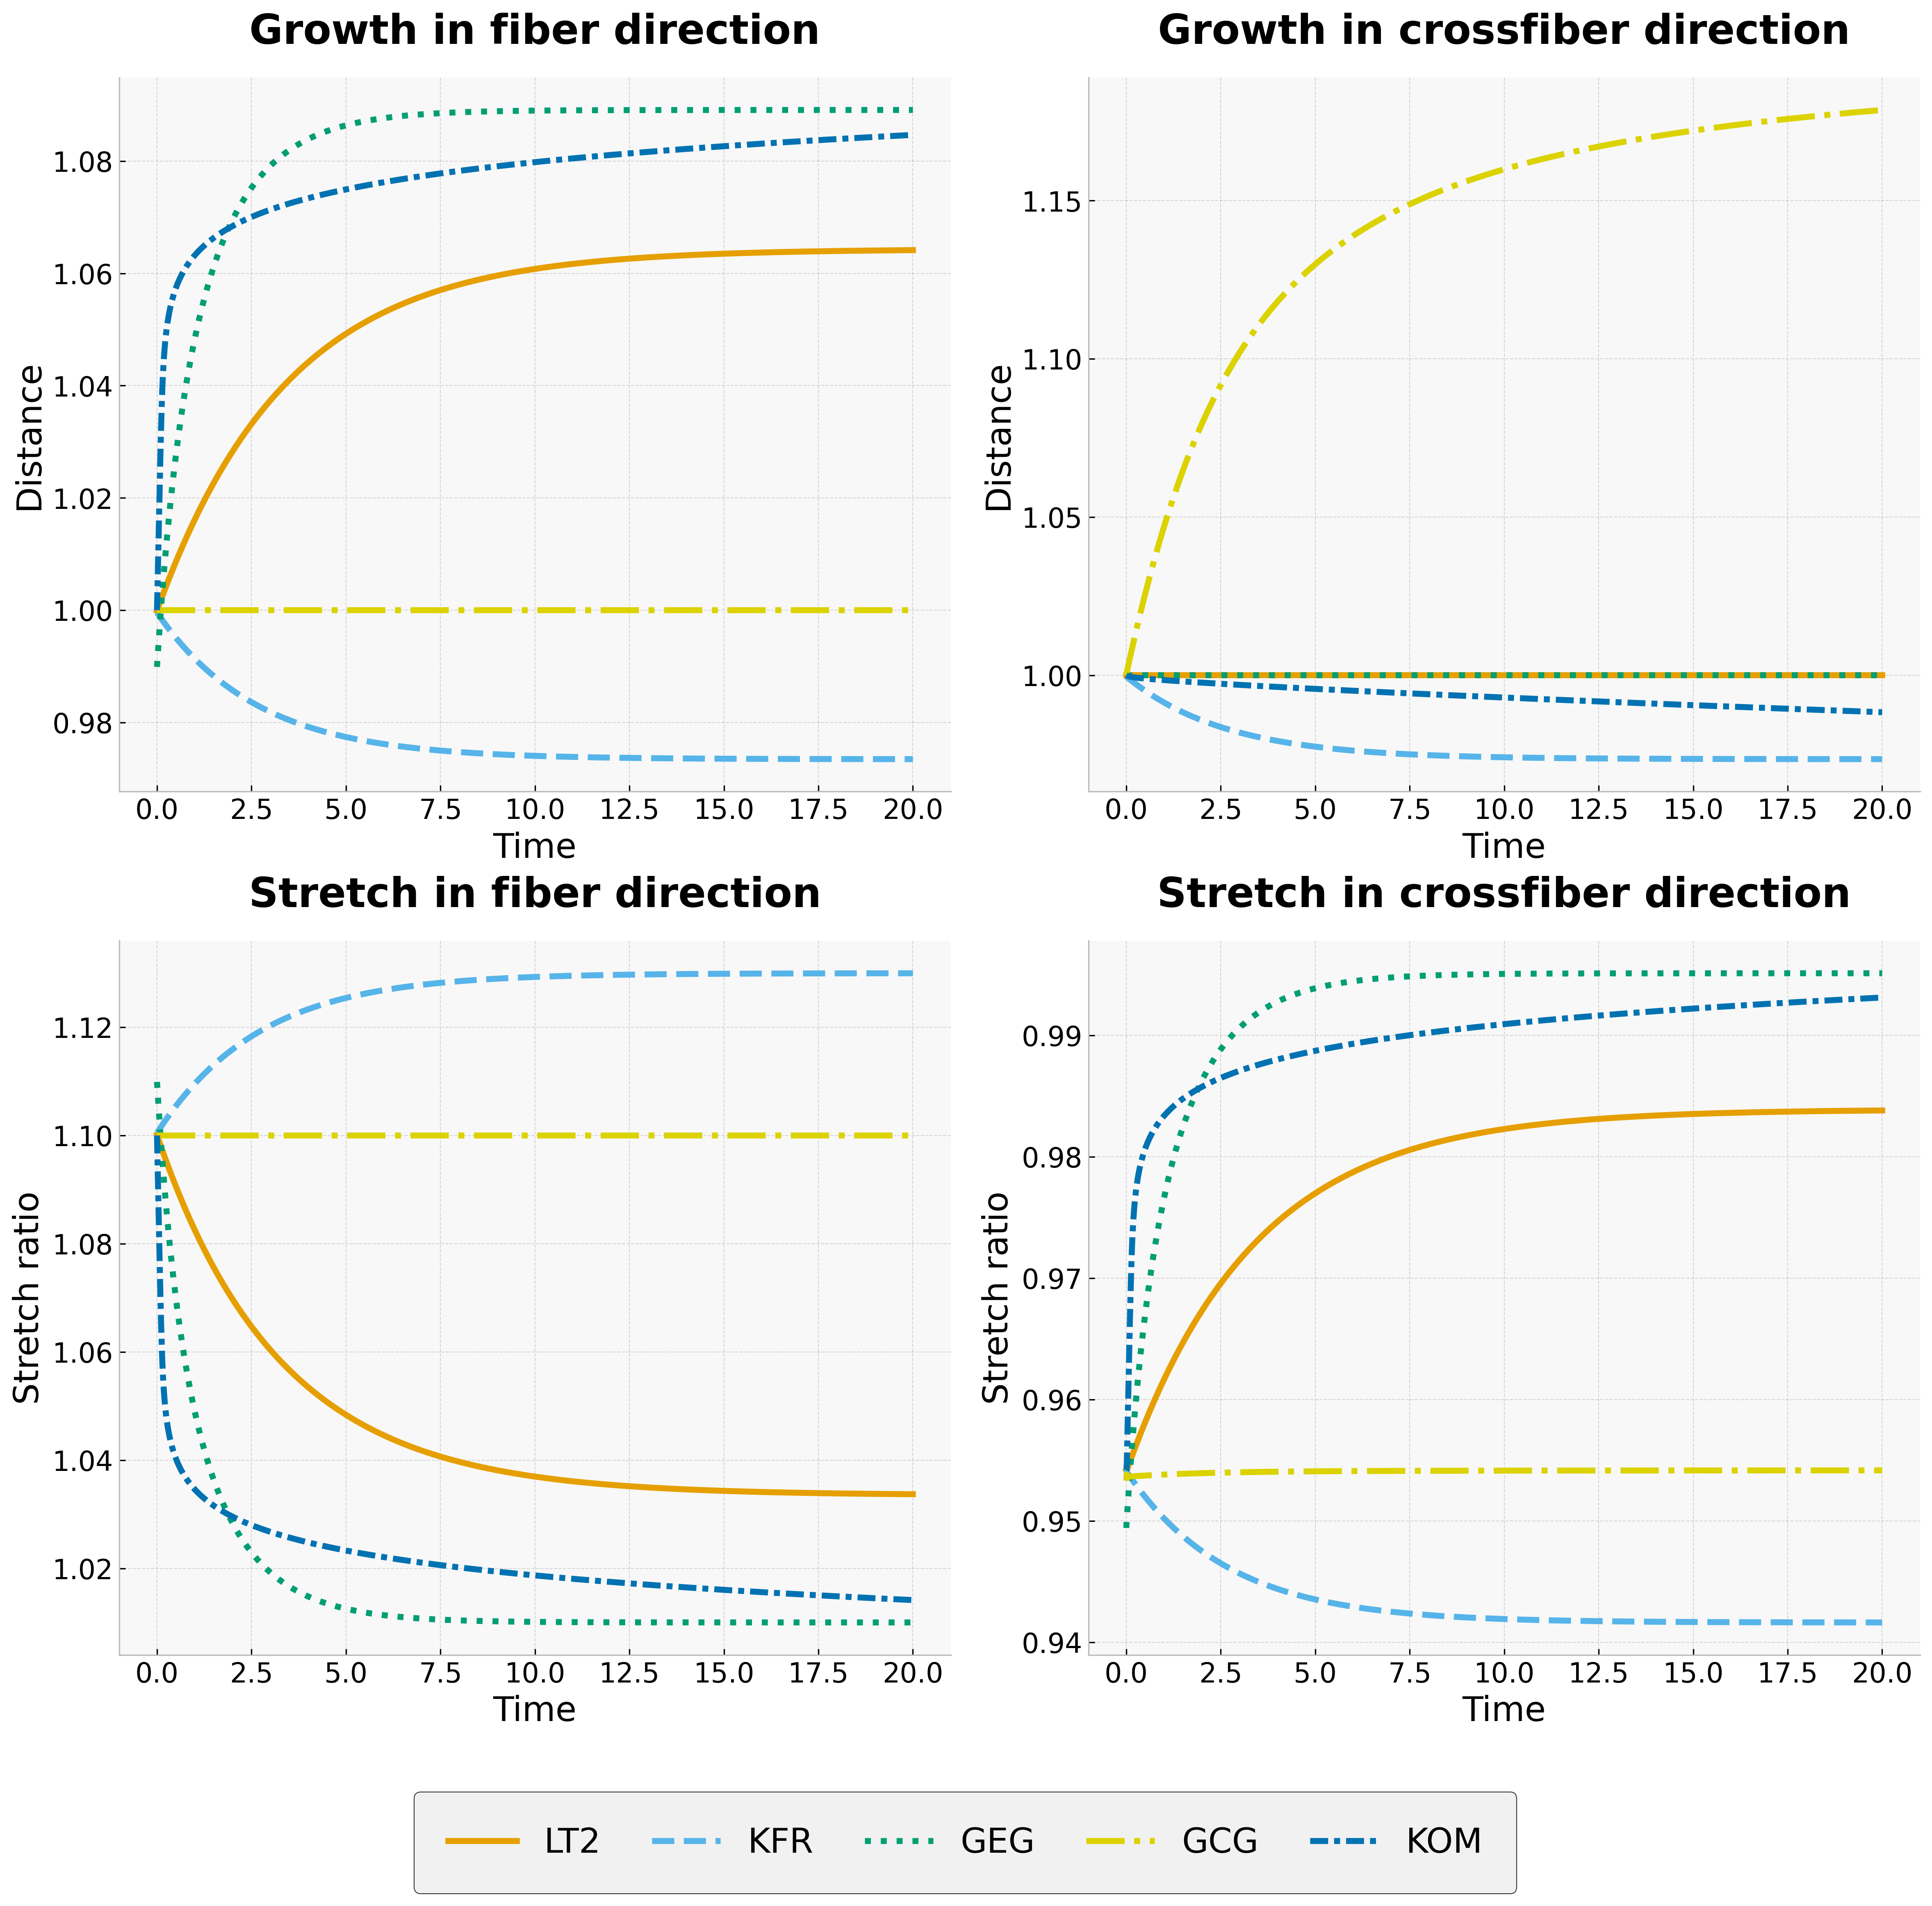
\includegraphics[width=\textwidth]{10p_stretch_3.png}
    \caption{Growth and stretch predicted by a 10\% stretch in the fiber direction.}
    \label{fig:10p_stretch}
\end{figure}
\begin{figure}[h]
    \centering
    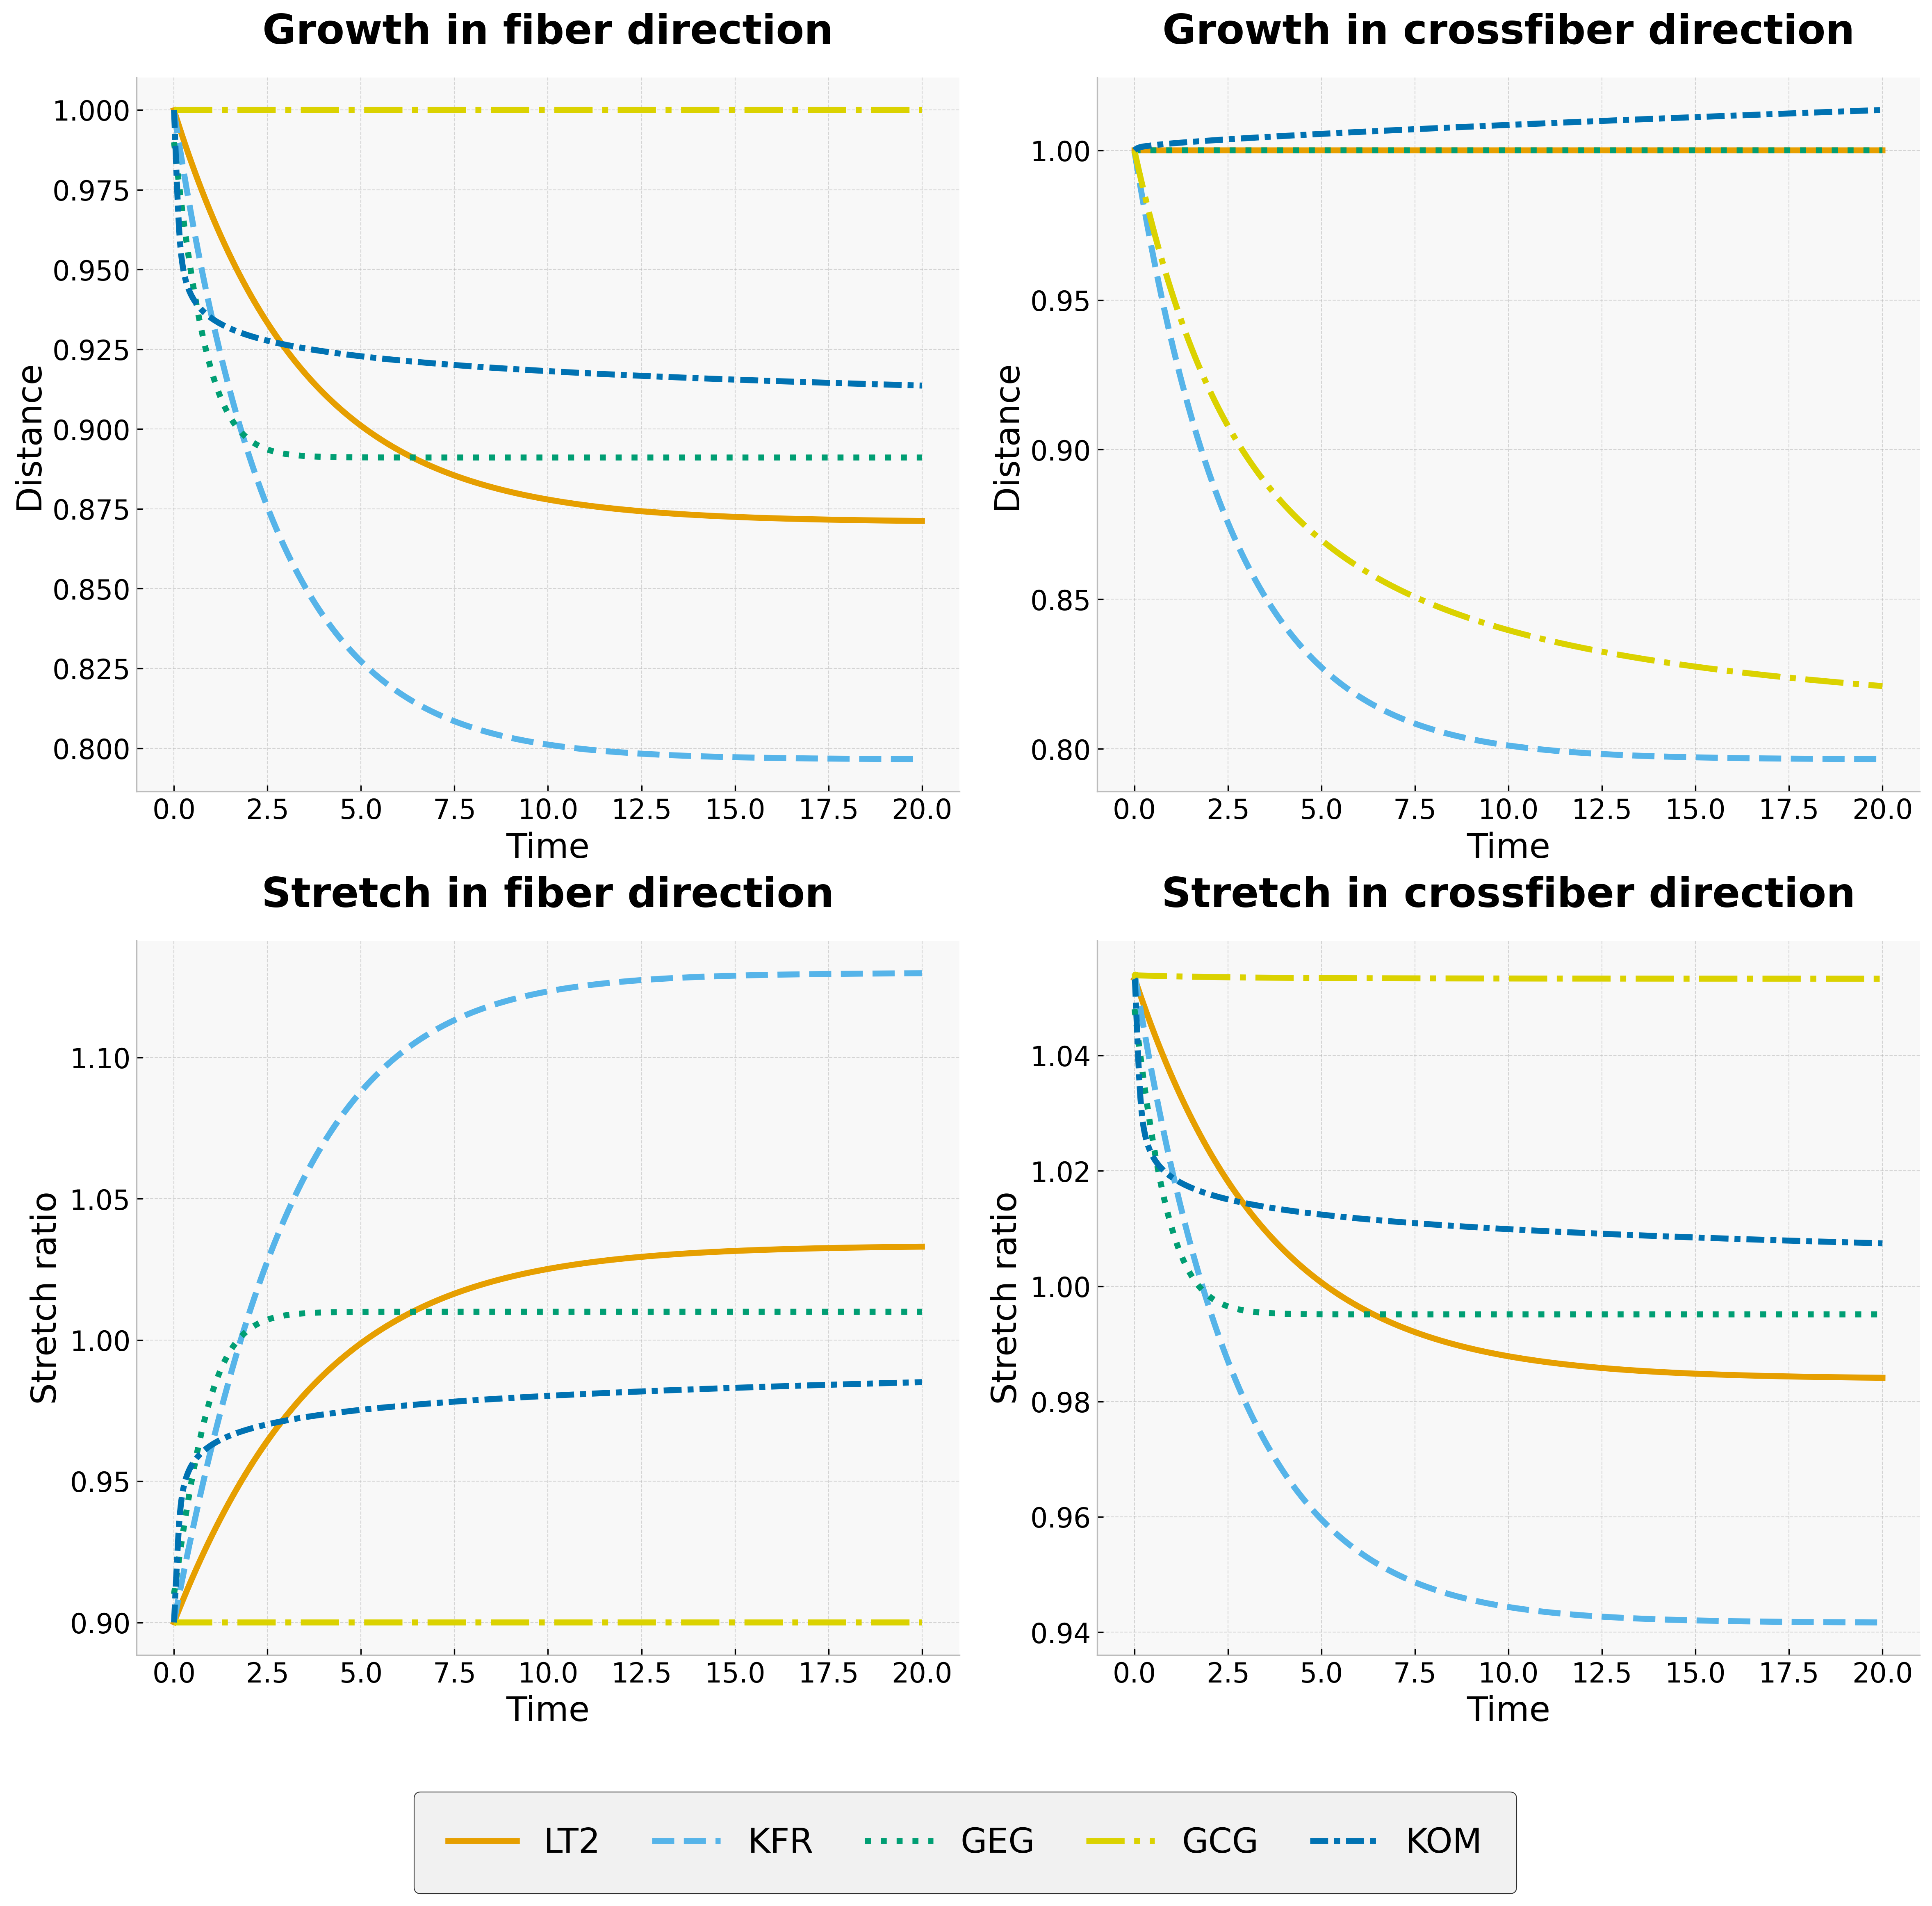
\includegraphics[width=\textwidth]{10p_compression_3.png}
    \caption{Growth and stretch predicted by a 10\% compression in the fiber direction.}
    \label{fig:10p_compression}
\end{figure}    

\section{Conclusion and future work}
We have implemented a general growth and remodelling framework using the FEniCSx program in Python. The goal is to easily change material models and growth models. This will allow researchers to compare their models with other models in the field. Future work will include implementing more complex geometries, more growth laws, and more material models. The models we have used in this paper are not derived from the dissipation equation but are instead phenomenologically derived growth laws and future work should investigate whether or not they satisfy the laws of thermodynamics. Another avenue of future research we wish to pursue is to look into constrained mixture models which model how changes in the various constituents influence the characteristics of the tissue. We also wish to add models that have more mathematically sophisticated stopping criteria, such as the ones developed by Erlich et al. \citep{Erlich2023} uses an energy penalty to construct a stopping criteria and \citep{Erlich2024} looks into how curvature\footnote{The intrinsic three dimensional curvature, not the two dimensional curvature of the surface of the body.} in the reference configuration could be used as a stopping criteria. Future work will also implement the growth models on geometries with fibers. We tried running the models on various fiber orientations and found them extremely sensitive to fibers that varied throughout the domain. Preliminary results indicate that some of the models do not converge to a steady state for relatively small perturbations of the variables or if the fibers are not well aligned with the body, something we plan on quantifying in the future. \par
When this package is further developed we aim to add it to the Pulse\footnote{https://github.com/finsberg/fenicsx-pulse} package. \par
The models we compared have been developed to capture different aspects of growth and were tuned to be used on different material models, so an apples-to-apples comparison might not be fair. Furthermore, the growth models we have used are not taking into account residual stresses that exist within the material before or after growth occurs. \par
Finally, experimental data is needed to verify which models are accurate or capture the correct phenomena of growing cardiac tissue.
% \newpage
\bibliographystyle{spbasic}
\bibliography{chapters/munthe/bibliography.bib}
% \printbibliography
% \end{document}
